\section{Design}

\subsection{UNO compontents}

My solution will be a LibreOffice extension that registers an UNO\cite{uno}
component. UNO is the interface based component model of LibreOffice. The main
feature it provides is that interfaces are defined in a language-idependent
IDL-like language, and they can be implemented in multiple languages:

\begin{itemize}
\item C
\item C++
\item Python
\item Java
\item BASIC
\end{itemize}

The caller is not aware which language the implementation uses, and it does not
need to, either. In my extension, I call BASIC macros from the menu elements,
which invoke the underlying Java code, where the business logic is implemented.

All the Java code is contained by a single jar file, the workflow of creating
it is the following:

\begin{figure}[H]
\centering
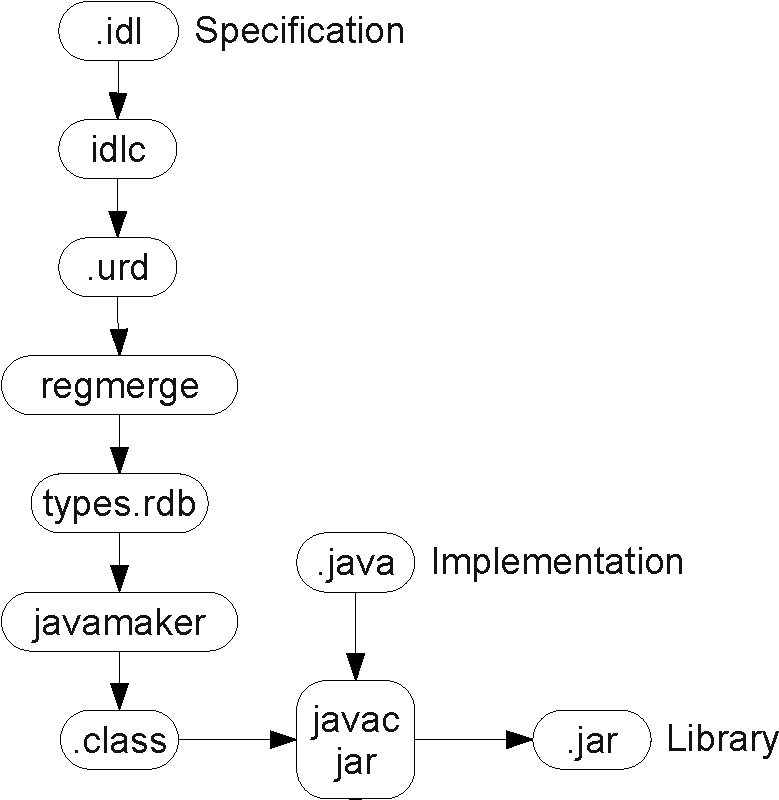
\includegraphics[width=250px,keepaspectratio]{uno-java.pdf}
\caption{Workflow of implementing an UNO service in Java}
\end{figure}

\begin{itemize}
\item \emph{idlc} compiles the .idl files to UNO Resource Descriptors,
\item \emph{regmerge} merges all the .urd files of the component to a single Resource Database,
\item \emph{javamaker} creates interfaces (.class files) from the Resource Database,
\item finally the standard Java development tools (\emph{javac}, \emph{jar})
creates the final jar, including the Java implementation.
\end{itemize}

Once the jar package is ready, a zip archive is created, containing:

\begin{itemize}
\item \emph{Addons.xcu}, containing the menu items
\item the BASIC library (callbacks for the menu items)
\item Java libraries used by the Java implementation
\item the Java implementation
\item metamodel of the stored settings
\item other files: metadata, extension description, license, etc.
\end{itemize}

Now that we saw the concept of UNO components and the structure of an
extension, the rest of this section describes the design of the UNO
specifications and Java implementations provided by the extension.

\subsection{The Sharepoint library}

At the time of writing, there is no ready to use Java library to communicate
with a Sharepoint server. Because of this, I decided to separate the Sharepoint
protocol implementation from the LibreOffice-specific part of the extension to
make it reusable in other projects. It provides the following features:

\begin{itemize}
\item \emph{Handler}: Handles requests from a frontend. Unless a feature has a
specific class, it is implemented here.
\item \emph{PacketParser}: Extracts the error message from a Vermeer
RPC\cite{vermeer} response packet.
\item \emph{FileOpenRootParser}: Parses the result from the \emph{list
workspaces} request.
\item \emph{FileOpenParser}: Parses the result from the \emph{list directory of
a workspace} request.
\item \emph{LastModParser}: Parses the result from the \emph{get last
modification date} request.
\item \emph{Version}: Handles document versions.
\item \emph{Messages}: Provides localization for the library error messages.
\item \emph{HandlerTest}: Automatically tests all features on a given server
using JUnit.
\end{itemize}
